\chapter{Resultados}
\label{cap:resultados}

Como abordado no Capítulo \ref{cap:desenvolvimento}, os métodos de validação com execução simbólica e o SSIP foram implementados a partir do jogo \textit{Shooterman} criado a fim de analisar estes métodos e estudar seus comportamentos e aplicações.
Todos experimentos foram executados 10 vezes, de onde obteve-se uma média aritmética de seus tempos de execução. Ambos métodos foram avaliados utilizando uma estrutura de arquivo contendo a sequência de ações realizadas por um cliente, facilitando assim o acesso aos dados de tempo de execução do processamento de validação em si, desconsiderando-se as falha de pacotes, latência da rede e outras características que poderiam alterar o tempo total de execução do método.

A máquina usada para os experimentos possui um processador \textit{quad-core} Intel(R) i5-2500 CPU, com 3.30GHz. O sistema operacional utilizado foi o Debian 4.6.2-2. A versão do compilador gcc utilizada foi a 6, e a do clang foi a 3.4.
Para gerar sequências de mensagens inválidas, alterou-se os arquivos de sequências de ações salvas durante uma sessão do jogo \textit{Shooterman}, adicionando ações de ativação de barreira e ativação de tiros em situações que não poderiam ser ativadas. Mudanças como múltiplas ações em uma única mensagem enviada também foram implantadas nos arquivos.

Ambos métodos conseguiram encontrar trapaças em todas as sequências de ações experimentadas. Em situações onde, por exemplo, o usuário atira em um intervalo de tempo que deveria ser proibido pela regras da aplicação, ambos métodos conseguiram reconhecer a trapaça. Situações semelhantes aconteceram quando o usuário tentou ativar seu escudo em momentos que ele estava em tempo de recarga. Outras trapaças, como modificação inválida da posição do jogador também foram reconhecidas pelos métodos.

Para a obtenção do tempo de execução da verificação de execução simbólica, foi utilizado o comando \textit{time} durante o período de execução do programa.
Para a verificação com o sistema de auditoria, foi utilizada a biblioteca \textit{chrono} do C++, possibilitando calcular somente o tempo de processamento das verificações, desconsiderando-se o tempo de leitura do arquivo com as ações verificadas. Esta estratégia foi adotada para ser mais fiel ao protocolo de auditoria, onde o processamento de verificação dos estados do cliente não acontece sobre arquivos armazenados no disco, mas sim sobre os dados já armazenados em memória. 



\section{Resultados da Execução Simbólica aplicada em Shooterman}

Percebe-se que apesar de ser uma implementação simples de execução simbólica, o tempo de execução de verificação das mensagens aumentou consideravelmente de acordo com o número de verificações realizadas. Isto provavelmente se deve ao fato de existir uma quantidade significativa de restrições existentes repetindo o mesmo fluxo de processamento executado pelas restrições anteriores. Ou seja, quando uma terceira ação vai ser validada, por exemplo, o mesmo processo de validação da primeira ação e da segunda ação que já foram calculados, são calculados novamente. 

Para uma sequência pequena a ser validada de 100 ações, o tempo de execução para a comparação foi de 1.5 segundos, valor já considerado alto para uma pequena quantidade de dados. Conforme o número de ações a ser validado aumenta, como o Gráfico \ref{fig:resultsimb} ilustra, o tempo de validação aumenta drasticamente, principalmente após a marca de 600 ações, onde a etapa de validação chega a passar de três minutos. 
Pode-se concluir que quanto mais restrições geradas pela execução simbólica, maior se torna o custo para computar seus próximos ramos. Uma solução para otimizar o custo para resolver de uma sequência grande de restrições pode ser a alteração do algoritmo resolvedor de restrições STP, visando reduzir o número de execuções duplicadas dos ramos. Outra estratégia que pode ser adotada para melhorar o desempenho da execução simbólica na validação das ações de um cliente é a verificação de sequências menores de ações. Como o número de restrições acaba sendo menor, o tempo total acaba sendo bem menor comparado a sequências maiores, como as apresentadas neste trabalho. 

Caso o verificador encontre uma sequência de mensagens inválidas, ele automaticamente para por não encontrar nenhum ramo de execução válido para seguir a computação. Esta abordagem para verificar as mensagens não se mostrou otimizada, e requer outras abordagens para ter um custo computacional menor para ser relevante na verificação de mensagens de jogos \textit{online}.

\begin{grafico}[h!]
	\begin{center}
		\scalebox{0.8}{
			% GNUPLOT: LaTeX picture with Postscript
\begingroup
  \makeatletter
  \providecommand\color[2][]{%
    \GenericError{(gnuplot) \space\space\space\@spaces}{%
      Package color not loaded in conjunction with
      terminal option `colourtext'%
    }{See the gnuplot documentation for explanation.%
    }{Either use 'blacktext' in gnuplot or load the package
      color.sty in LaTeX.}%
    \renewcommand\color[2][]{}%
  }%
  \providecommand\includegraphics[2][]{%
    \GenericError{(gnuplot) \space\space\space\@spaces}{%
      Package graphicx or graphics not loaded%
    }{See the gnuplot documentation for explanation.%
    }{The gnuplot epslatex terminal needs graphicx.sty or graphics.sty.}%
    \renewcommand\includegraphics[2][]{}%
  }%
  \providecommand\rotatebox[2]{#2}%
  \@ifundefined{ifGPcolor}{%
    \newif\ifGPcolor
    \GPcolorfalse
  }{}%
  \@ifundefined{ifGPblacktext}{%
    \newif\ifGPblacktext
    \GPblacktexttrue
  }{}%
  % define a \g@addto@macro without @ in the name:
  \let\gplgaddtomacro\g@addto@macro
  % define empty templates for all commands taking text:
  \gdef\gplbacktext{}%
  \gdef\gplfronttext{}%
  \makeatother
  \ifGPblacktext
    % no textcolor at all
    \def\colorrgb#1{}%
    \def\colorgray#1{}%
  \else
    % gray or color?
    \ifGPcolor
      \def\colorrgb#1{\color[rgb]{#1}}%
      \def\colorgray#1{\color[gray]{#1}}%
      \expandafter\def\csname LTw\endcsname{\color{white}}%
      \expandafter\def\csname LTb\endcsname{\color{black}}%
      \expandafter\def\csname LTa\endcsname{\color{black}}%
      \expandafter\def\csname LT0\endcsname{\color[rgb]{1,0,0}}%
      \expandafter\def\csname LT1\endcsname{\color[rgb]{0,1,0}}%
      \expandafter\def\csname LT2\endcsname{\color[rgb]{0,0,1}}%
      \expandafter\def\csname LT3\endcsname{\color[rgb]{1,0,1}}%
      \expandafter\def\csname LT4\endcsname{\color[rgb]{0,1,1}}%
      \expandafter\def\csname LT5\endcsname{\color[rgb]{1,1,0}}%
      \expandafter\def\csname LT6\endcsname{\color[rgb]{0,0,0}}%
      \expandafter\def\csname LT7\endcsname{\color[rgb]{1,0.3,0}}%
      \expandafter\def\csname LT8\endcsname{\color[rgb]{0.5,0.5,0.5}}%
    \else
      % gray
      \def\colorrgb#1{\color{black}}%
      \def\colorgray#1{\color[gray]{#1}}%
      \expandafter\def\csname LTw\endcsname{\color{white}}%
      \expandafter\def\csname LTb\endcsname{\color{black}}%
      \expandafter\def\csname LTa\endcsname{\color{black}}%
      \expandafter\def\csname LT0\endcsname{\color{black}}%
      \expandafter\def\csname LT1\endcsname{\color{black}}%
      \expandafter\def\csname LT2\endcsname{\color{black}}%
      \expandafter\def\csname LT3\endcsname{\color{black}}%
      \expandafter\def\csname LT4\endcsname{\color{black}}%
      \expandafter\def\csname LT5\endcsname{\color{black}}%
      \expandafter\def\csname LT6\endcsname{\color{black}}%
      \expandafter\def\csname LT7\endcsname{\color{black}}%
      \expandafter\def\csname LT8\endcsname{\color{black}}%
    \fi
  \fi
    \setlength{\unitlength}{0.0500bp}%
    \ifx\gptboxheight\undefined%
      \newlength{\gptboxheight}%
      \newlength{\gptboxwidth}%
      \newsavebox{\gptboxtext}%
    \fi%
    \setlength{\fboxrule}{0.5pt}%
    \setlength{\fboxsep}{1pt}%
\begin{picture}(7200.00,5040.00)%
    \gplgaddtomacro\gplbacktext{%
      \csname LTb\endcsname%
      \put(814,704){\makebox(0,0)[r]{\strut{}$0$}}%
      \csname LTb\endcsname%
      \put(814,1213){\makebox(0,0)[r]{\strut{}$100$}}%
      \csname LTb\endcsname%
      \put(814,1722){\makebox(0,0)[r]{\strut{}$200$}}%
      \csname LTb\endcsname%
      \put(814,2231){\makebox(0,0)[r]{\strut{}$300$}}%
      \csname LTb\endcsname%
      \put(814,2740){\makebox(0,0)[r]{\strut{}$400$}}%
      \csname LTb\endcsname%
      \put(814,3248){\makebox(0,0)[r]{\strut{}$500$}}%
      \csname LTb\endcsname%
      \put(814,3757){\makebox(0,0)[r]{\strut{}$600$}}%
      \csname LTb\endcsname%
      \put(814,4266){\makebox(0,0)[r]{\strut{}$700$}}%
      \csname LTb\endcsname%
      \put(814,4775){\makebox(0,0)[r]{\strut{}$800$}}%
      \put(946,484){\makebox(0,0){\strut{}$128$}}%
      \put(2898,484){\makebox(0,0){\strut{}$256$}}%
      \put(4851,484){\makebox(0,0){\strut{}$512$}}%
      \put(6803,484){\makebox(0,0){\strut{}$1024$}}%
    }%
    \gplgaddtomacro\gplfronttext{%
      \csname LTb\endcsname%
      \put(176,2739){\rotatebox{-270}{\makebox(0,0){\strut{}tempo de execução(s)}}}%
      \put(3874,154){\makebox(0,0){\strut{}nº mensagens}}%
      \csname LTb\endcsname%
      \put(3300,4461){\makebox(0,0)[r]{\strut{}Execução Simbólica}}%
    }%
    \gplbacktext
    \put(0,0){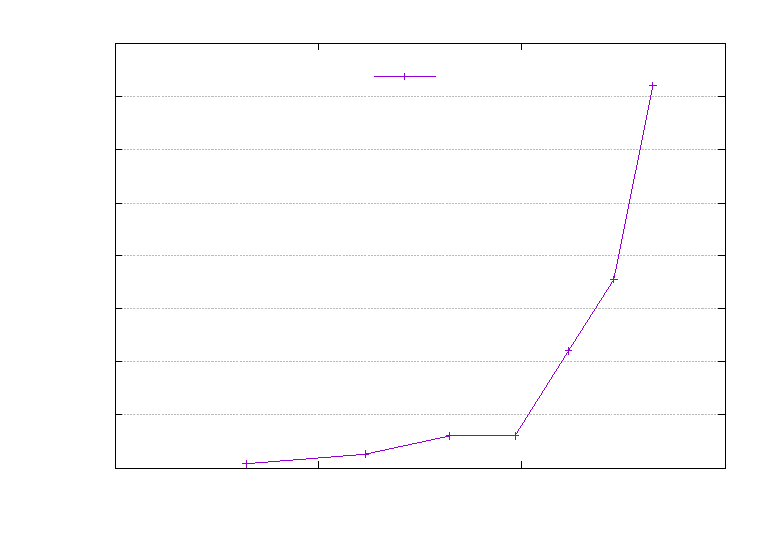
\includegraphics{simbolic}}%
    \gplfronttext
  \end{picture}%
\endgroup
		
			}
		\caption[Resultados obtidos com verificação por execução simbólica.]{Resultados obtidos com validação por execução simbólica.}
		\label{fig:resultsimb}	
	\end{center}

\end{grafico}

\section{Resultados do SSIP aplicado em Shooterman}

Os resultados do protocolo de integridade semântica segura mostraram-se eficientes. Como o Gráfico \label{fig:resultaudit} demonstra, o método conseguiu verificar grandes quantidades de blocos de ações em um curto período de tempo. Para sequências de mensagens com tamanho inferior a 20000, o tempo de execução das verificações foi na escala de microsegundos, com 23 microsegundos de execução tanto para sequências de 10000 e 20000 mensagens. O tempo começou a aumentar em sequências maiores, mas ainda se manteve sempre próximo da faixa de tempo de um segundo. Percebe-se que a cada 10000 novas mensagens a serem processadas, o tempo de execução aumenta aproximadamente 0,15 segundos, mantendo-se em um crescimento linear.  

\begin{grafico}[h!]
	\begin{center}
			%\scalebox{0.8}{
	%		% GNUPLOT: LaTeX picture with Postscript
\begingroup
  \makeatletter
  \providecommand\color[2][]{%
    \GenericError{(gnuplot) \space\space\space\@spaces}{%
      Package color not loaded in conjunction with
      terminal option `colourtext'%
    }{See the gnuplot documentation for explanation.%
    }{Either use 'blacktext' in gnuplot or load the package
      color.sty in LaTeX.}%
    \renewcommand\color[2][]{}%
  }%
  \providecommand\includegraphics[2][]{%
    \GenericError{(gnuplot) \space\space\space\@spaces}{%
      Package graphicx or graphics not loaded%
    }{See the gnuplot documentation for explanation.%
    }{The gnuplot epslatex terminal needs graphicx.sty or graphics.sty.}%
    \renewcommand\includegraphics[2][]{}%
  }%
  \providecommand\rotatebox[2]{#2}%
  \@ifundefined{ifGPcolor}{%
    \newif\ifGPcolor
    \GPcolorfalse
  }{}%
  \@ifundefined{ifGPblacktext}{%
    \newif\ifGPblacktext
    \GPblacktexttrue
  }{}%
  % define a \g@addto@macro without @ in the name:
  \let\gplgaddtomacro\g@addto@macro
  % define empty templates for all commands taking text:
  \gdef\gplbacktext{}%
  \gdef\gplfronttext{}%
  \makeatother
  \ifGPblacktext
    % no textcolor at all
    \def\colorrgb#1{}%
    \def\colorgray#1{}%
  \else
    % gray or color?
    \ifGPcolor
      \def\colorrgb#1{\color[rgb]{#1}}%
      \def\colorgray#1{\color[gray]{#1}}%
      \expandafter\def\csname LTw\endcsname{\color{white}}%
      \expandafter\def\csname LTb\endcsname{\color{black}}%
      \expandafter\def\csname LTa\endcsname{\color{black}}%
      \expandafter\def\csname LT0\endcsname{\color[rgb]{1,0,0}}%
      \expandafter\def\csname LT1\endcsname{\color[rgb]{0,1,0}}%
      \expandafter\def\csname LT2\endcsname{\color[rgb]{0,0,1}}%
      \expandafter\def\csname LT3\endcsname{\color[rgb]{1,0,1}}%
      \expandafter\def\csname LT4\endcsname{\color[rgb]{0,1,1}}%
      \expandafter\def\csname LT5\endcsname{\color[rgb]{1,1,0}}%
      \expandafter\def\csname LT6\endcsname{\color[rgb]{0,0,0}}%
      \expandafter\def\csname LT7\endcsname{\color[rgb]{1,0.3,0}}%
      \expandafter\def\csname LT8\endcsname{\color[rgb]{0.5,0.5,0.5}}%
    \else
      % gray
      \def\colorrgb#1{\color{black}}%
      \def\colorgray#1{\color[gray]{#1}}%
      \expandafter\def\csname LTw\endcsname{\color{white}}%
      \expandafter\def\csname LTb\endcsname{\color{black}}%
      \expandafter\def\csname LTa\endcsname{\color{black}}%
      \expandafter\def\csname LT0\endcsname{\color{black}}%
      \expandafter\def\csname LT1\endcsname{\color{black}}%
      \expandafter\def\csname LT2\endcsname{\color{black}}%
      \expandafter\def\csname LT3\endcsname{\color{black}}%
      \expandafter\def\csname LT4\endcsname{\color{black}}%
      \expandafter\def\csname LT5\endcsname{\color{black}}%
      \expandafter\def\csname LT6\endcsname{\color{black}}%
      \expandafter\def\csname LT7\endcsname{\color{black}}%
      \expandafter\def\csname LT8\endcsname{\color{black}}%
    \fi
  \fi
    \setlength{\unitlength}{0.0500bp}%
    \ifx\gptboxheight\undefined%
      \newlength{\gptboxheight}%
      \newlength{\gptboxwidth}%
      \newsavebox{\gptboxtext}%
    \fi%
    \setlength{\fboxrule}{0.5pt}%
    \setlength{\fboxsep}{1pt}%
\begin{picture}(7200.00,5040.00)%
    \gplgaddtomacro\gplbacktext{%
      \csname LTb\endcsname%
      \put(814,704){\makebox(0,0)[r]{\strut{}$0$}}%
      \csname LTb\endcsname%
      \put(814,1213){\makebox(0,0)[r]{\strut{}$0.1$}}%
      \csname LTb\endcsname%
      \put(814,1722){\makebox(0,0)[r]{\strut{}$0.2$}}%
      \csname LTb\endcsname%
      \put(814,2231){\makebox(0,0)[r]{\strut{}$0.3$}}%
      \csname LTb\endcsname%
      \put(814,2740){\makebox(0,0)[r]{\strut{}$0.4$}}%
      \csname LTb\endcsname%
      \put(814,3248){\makebox(0,0)[r]{\strut{}$0.5$}}%
      \csname LTb\endcsname%
      \put(814,3757){\makebox(0,0)[r]{\strut{}$0.6$}}%
      \csname LTb\endcsname%
      \put(814,4266){\makebox(0,0)[r]{\strut{}$0.7$}}%
      \csname LTb\endcsname%
      \put(814,4775){\makebox(0,0)[r]{\strut{}$0.8$}}%
      \put(946,484){\makebox(0,0){\strut{}$20000$}}%
      \put(1922,484){\makebox(0,0){\strut{}$30000$}}%
      \put(2898,484){\makebox(0,0){\strut{}$40000$}}%
      \put(3875,484){\makebox(0,0){\strut{}$50000$}}%
      \put(4851,484){\makebox(0,0){\strut{}$60000$}}%
      \put(5827,484){\makebox(0,0){\strut{}$70000$}}%
      \put(6803,484){\makebox(0,0){\strut{}$80000$}}%
    }%
    \gplgaddtomacro\gplfronttext{%
      \csname LTb\endcsname%
      \put(176,2739){\rotatebox{-270}{\makebox(0,0){\strut{}tempo de execução(s)}}}%
      \put(3874,154){\makebox(0,0){\strut{}nº mensagens}}%
      \csname LTb\endcsname%
      \put(-1825,3868044){\makebox(0,0)[r]{\strut{}Auditoria}}%
    }%
    \gplbacktext
    \put(0,0){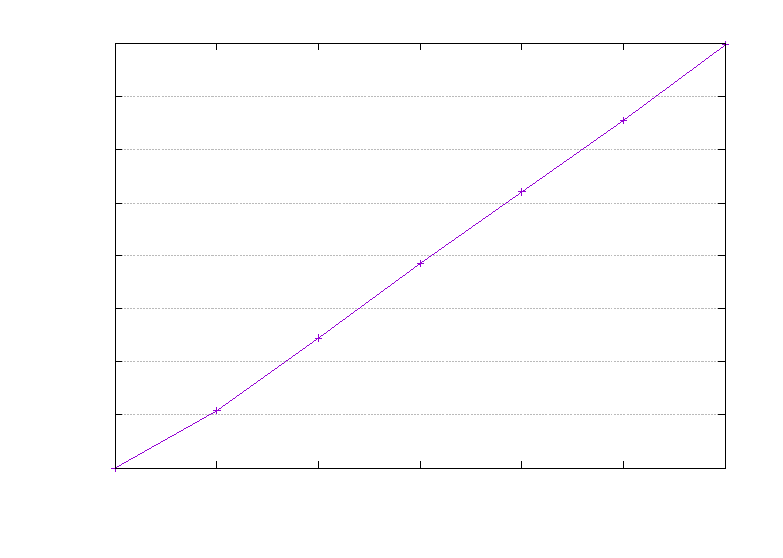
\includegraphics{auditoria}}%
    \gplfronttext
  \end{picture}%
\endgroup
		
	%		}
	    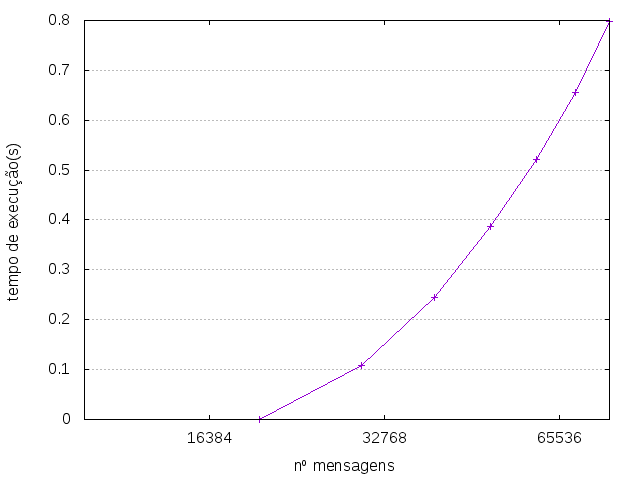
\includegraphics[width=0.65\textwidth]{imagens/auditoria.png}
		\caption[Resultados obtidos com validação com auditoria.]{Resultados obtidos com validação com auditoria.}
		\label{fig:resultaudit}	
	\end{center}

\end{grafico}



Em um cenário convencional, dificilmente o servidor de auditoria precisaria avaliar sequências tão grandes de ações executadas pelo cliente. Mesmo assim, o algoritmo do protocolo mostrou-se eficiente para lidar com sequências de até mesmo 80000 ações. Comparando com os resultados obtidos da verificação de mensagens utilizando execução simbólica, o SSIP mostrou-se muito superior em questões de desempenho de tempo de execução. Além de mostrar-se eficiente na verificação das ações de \textit{Shooterman}, o protocolo mostra-se versátil por dar a opção do desenvolvedor escolher de quantos em quantos ciclos de um cliente inicia-se um processo de auditoria. Além disso, como apenas uma auditoria é feita com um cliente por vez, o processamento gasto pelo servidor de auditoria acaba sendo bem reduzido. No geral, o SSIP mostrou-se interessante para verificar a integridade de mensagens.

Entretanto, algumas características negativas podem ser atribuídas ao SSIP. Considerando que, a cada ciclo do cliente ele envia informações adicionais contendo as mudanças concretas de seus estados ao servidor de auditoria, o número de mensagens a ser enviadas dobra. Além de enviar as alterações abstratas ao servidor da aplicação, as alterações concretas (que possuem tamanhos maiores de mensagens) também são enviadas. Pode-se afirmar, que em média, o tamanho das mensagens do SSIP é o dobro do convencional, pela duplicidade das informações enviadas tanto ao servidor principal como ao servidor de auditoria.

